\documentclass[twoside]{book}

% Packages required by doxygen
\usepackage{fixltx2e}
\usepackage{calc}
\usepackage{doxygen}
\usepackage[export]{adjustbox} % also loads graphicx
\usepackage{graphicx}
\usepackage[utf8]{inputenc}
\usepackage{makeidx}
\usepackage{multicol}
\usepackage{multirow}
\PassOptionsToPackage{warn}{textcomp}
\usepackage{textcomp}
\usepackage[nointegrals]{wasysym}
\usepackage[table]{xcolor}

% Font selection
\usepackage[T1]{fontenc}
\usepackage[scaled=.90]{helvet}
\usepackage{courier}
\usepackage{amssymb}
\usepackage{sectsty}
\renewcommand{\familydefault}{\sfdefault}
\allsectionsfont{%
  \fontseries{bc}\selectfont%
  \color{darkgray}%
}
\renewcommand{\DoxyLabelFont}{%
  \fontseries{bc}\selectfont%
  \color{darkgray}%
}
\newcommand{\+}{\discretionary{\mbox{\scriptsize$\hookleftarrow$}}{}{}}

% Page & text layout
\usepackage{geometry}
\geometry{%
  a4paper,%
  top=2.5cm,%
  bottom=2.5cm,%
  left=2.5cm,%
  right=2.5cm%
}
\tolerance=750
\hfuzz=15pt
\hbadness=750
\setlength{\emergencystretch}{15pt}
\setlength{\parindent}{0cm}
\setlength{\parskip}{0.2cm}
\makeatletter
\renewcommand{\paragraph}{%
  \@startsection{paragraph}{4}{0ex}{-1.0ex}{1.0ex}{%
    \normalfont\normalsize\bfseries\SS@parafont%
  }%
}
\renewcommand{\subparagraph}{%
  \@startsection{subparagraph}{5}{0ex}{-1.0ex}{1.0ex}{%
    \normalfont\normalsize\bfseries\SS@subparafont%
  }%
}
\makeatother

% Headers & footers
\usepackage{fancyhdr}
\pagestyle{fancyplain}
\fancyhead[LE]{\fancyplain{}{\bfseries\thepage}}
\fancyhead[CE]{\fancyplain{}{}}
\fancyhead[RE]{\fancyplain{}{\bfseries\leftmark}}
\fancyhead[LO]{\fancyplain{}{\bfseries\rightmark}}
\fancyhead[CO]{\fancyplain{}{}}
\fancyhead[RO]{\fancyplain{}{\bfseries\thepage}}
\fancyfoot[LE]{\fancyplain{}{}}
\fancyfoot[CE]{\fancyplain{}{}}
\fancyfoot[RE]{\fancyplain{}{\bfseries\scriptsize Generated on Fri Jun 12 2015 23\+:30\+:55 for My Project by Doxygen }}
\fancyfoot[LO]{\fancyplain{}{\bfseries\scriptsize Generated on Fri Jun 12 2015 23\+:30\+:55 for My Project by Doxygen }}
\fancyfoot[CO]{\fancyplain{}{}}
\fancyfoot[RO]{\fancyplain{}{}}
\renewcommand{\footrulewidth}{0.4pt}
\renewcommand{\chaptermark}[1]{%
  \markboth{#1}{}%
}
\renewcommand{\sectionmark}[1]{%
  \markright{\thesection\ #1}%
}

% Indices & bibliography
\usepackage{natbib}
\usepackage[titles]{tocloft}
\setcounter{tocdepth}{3}
\setcounter{secnumdepth}{5}
\makeindex

% Hyperlinks (required, but should be loaded last)
\usepackage{ifpdf}
\ifpdf
  \usepackage[pdftex,pagebackref=true]{hyperref}
\else
  \usepackage[ps2pdf,pagebackref=true]{hyperref}
\fi
\hypersetup{%
  colorlinks=true,%
  linkcolor=blue,%
  citecolor=blue,%
  unicode%
}

% Custom commands
\newcommand{\clearemptydoublepage}{%
  \newpage{\pagestyle{empty}\cleardoublepage}%
}


%===== C O N T E N T S =====

\begin{document}

% Titlepage & ToC
\hypersetup{pageanchor=false,
             bookmarks=true,
             bookmarksnumbered=true,
             pdfencoding=unicode
            }
\pagenumbering{roman}
\begin{titlepage}
\vspace*{7cm}
\begin{center}%
{\Large My Project }\\
\vspace*{1cm}
{\large Generated by Doxygen 1.8.9.1}\\
\vspace*{0.5cm}
{\small Fri Jun 12 2015 23:30:55}\\
\end{center}
\end{titlepage}
\clearemptydoublepage
\tableofcontents
\clearemptydoublepage
\pagenumbering{arabic}
\hypersetup{pageanchor=true}

%--- Begin generated contents ---
\chapter{Hierarchical Index}
\section{Class Hierarchy}
This inheritance list is sorted roughly, but not completely, alphabetically\+:\begin{DoxyCompactList}
\item \contentsline{section}{Abs\+Player}{\pageref{class_abs_player}}{}
\begin{DoxyCompactList}
\item \contentsline{section}{Player}{\pageref{class_player}}{}
\begin{DoxyCompactList}
\item \contentsline{section}{A\+I}{\pageref{class_a_i}}{}
\end{DoxyCompactList}
\end{DoxyCompactList}
\item \contentsline{section}{a\+Vector$<$ T $>$}{\pageref{classa_vector}}{}
\item \contentsline{section}{a\+Vector$<$ char $>$}{\pageref{classa_vector}}{}
\item \contentsline{section}{Info}{\pageref{struct_info}}{}
\end{DoxyCompactList}

\chapter{Class Index}
\section{Class List}
Here are the classes, structs, unions and interfaces with brief descriptions\+:\begin{DoxyCompactList}
\item\contentsline{section}{\hyperlink{class_abs_player}{Abs\+Player} }{\pageref{class_abs_player}}{}
\item\contentsline{section}{\hyperlink{class_a_i}{A\+I} }{\pageref{class_a_i}}{}
\item\contentsline{section}{\hyperlink{classa_vector}{a\+Vector$<$ T $>$} }{\pageref{classa_vector}}{}
\item\contentsline{section}{\hyperlink{struct_info}{Info} }{\pageref{struct_info}}{}
\item\contentsline{section}{\hyperlink{class_player}{Player} }{\pageref{class_player}}{}
\end{DoxyCompactList}

\chapter{Class Documentation}
\hypertarget{class_abs_player}{}\section{Abs\+Player Class Reference}
\label{class_abs_player}\index{Abs\+Player@{Abs\+Player}}
Inheritance diagram for Abs\+Player\+:\begin{figure}[H]
\begin{center}
\leavevmode
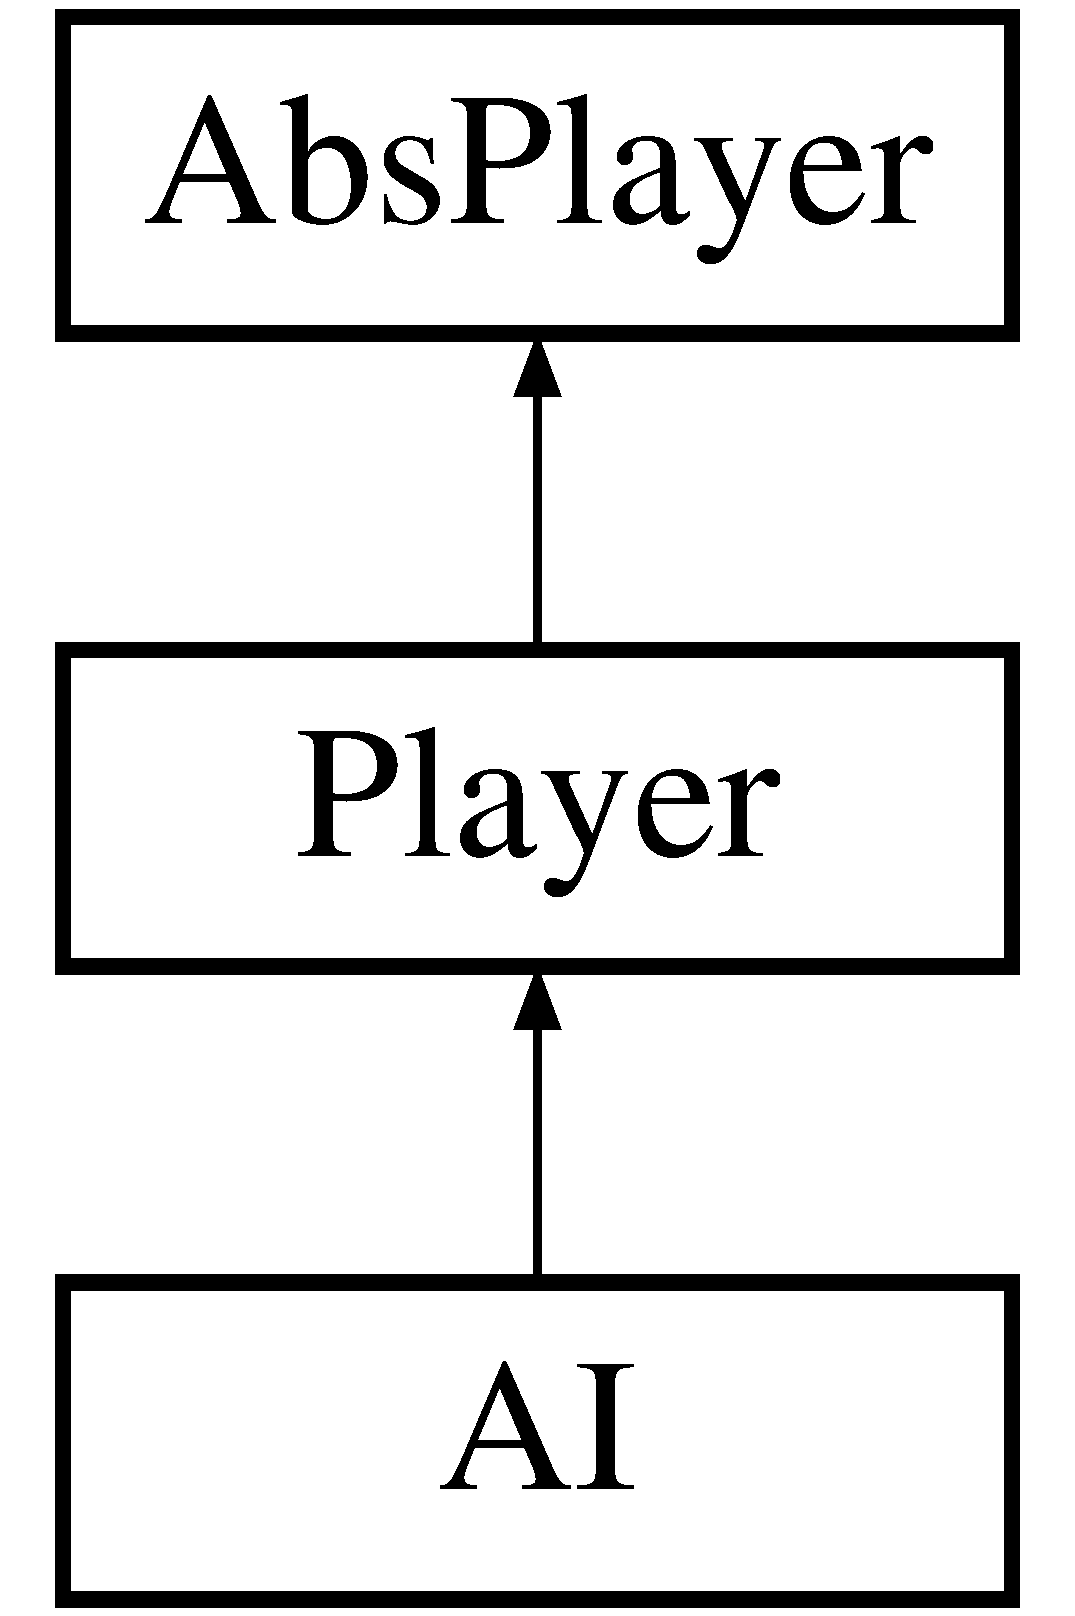
\includegraphics[height=3.000000cm]{class_abs_player}
\end{center}
\end{figure}
\subsection*{Public Member Functions}
\begin{DoxyCompactItemize}
\item 
\hypertarget{class_abs_player_afa4d8a2ff833bf9345435f5fc9edcb5b}{}virtual void {\bfseries bid} ()=0\label{class_abs_player_afa4d8a2ff833bf9345435f5fc9edcb5b}

\item 
\hypertarget{class_abs_player_ae6035f09728fc47c3647a6da318ea058}{}virtual void {\bfseries chalng} ()=0\label{class_abs_player_ae6035f09728fc47c3647a6da318ea058}

\end{DoxyCompactItemize}


\subsection{Detailed Description}


Definition at line 11 of file Abs\+Player.\+h.



The documentation for this class was generated from the following file\+:\begin{DoxyCompactItemize}
\item 
Abs\+Player.\+h\end{DoxyCompactItemize}

\hypertarget{class_a_i}{}\section{A\+I Class Reference}
\label{class_a_i}\index{A\+I@{A\+I}}
Inheritance diagram for A\+I\+:\begin{figure}[H]
\begin{center}
\leavevmode
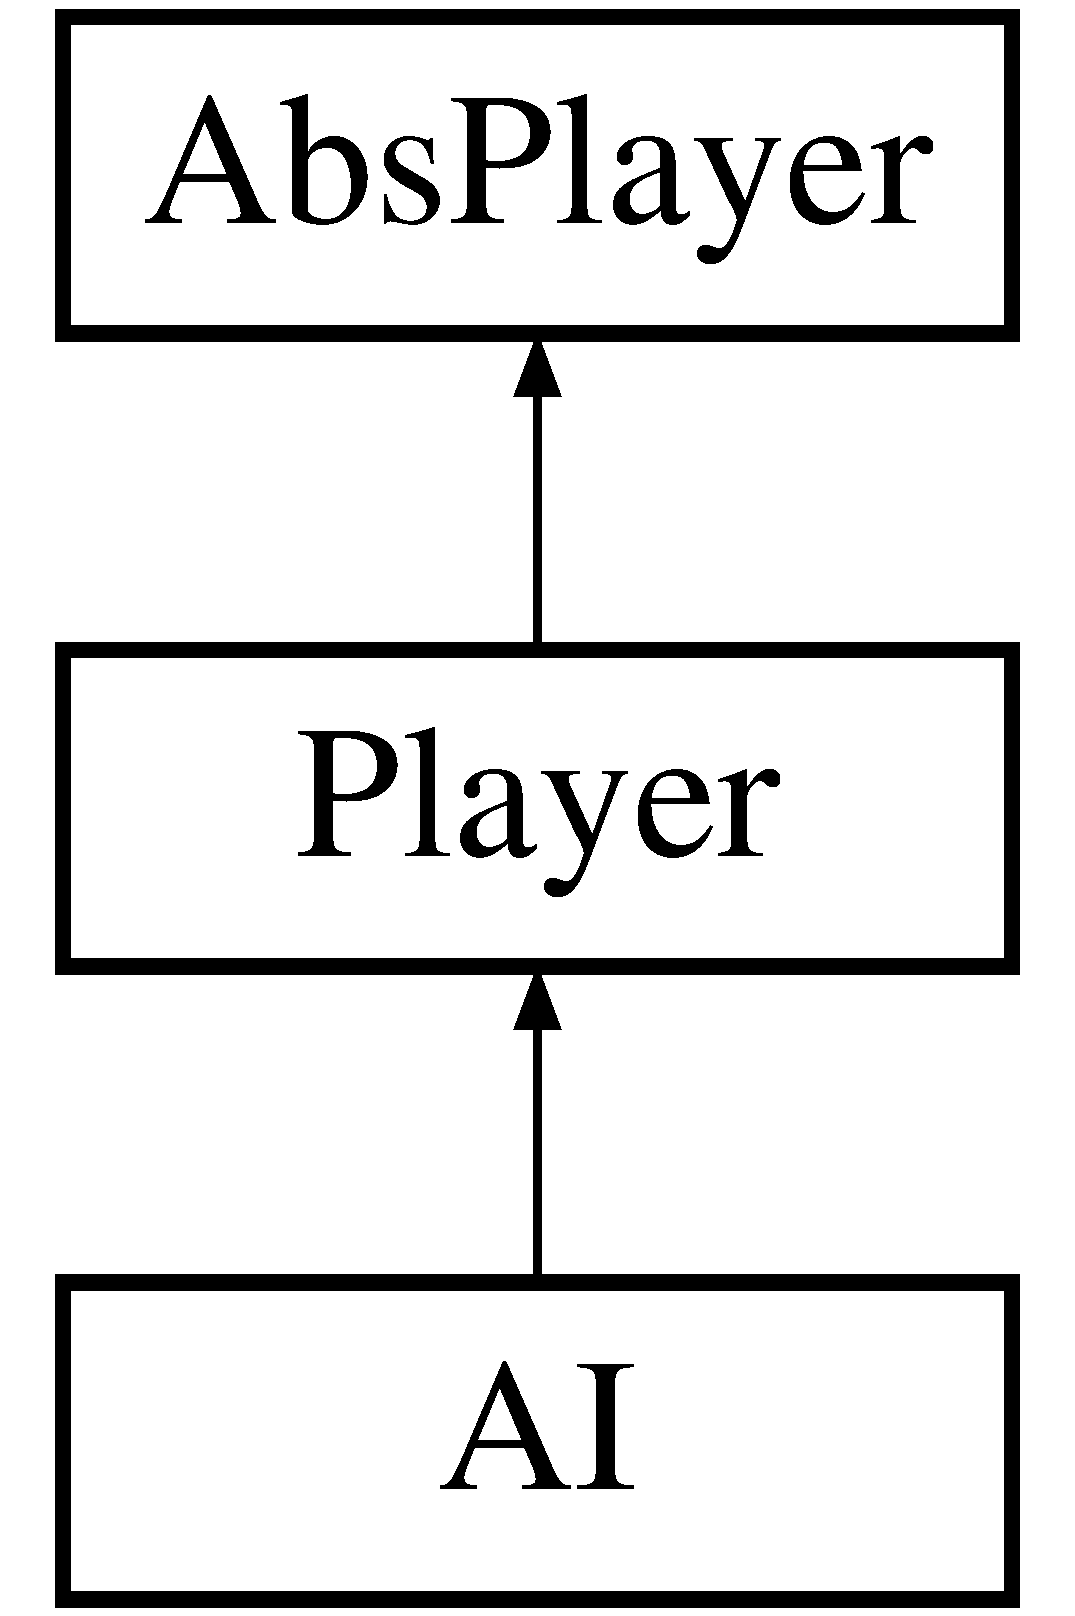
\includegraphics[height=3.000000cm]{class_a_i}
\end{center}
\end{figure}
\subsection*{Public Member Functions}
\begin{DoxyCompactItemize}
\item 
\hypertarget{class_a_i_afe998e179e8c6afd5a2248ecaf38c02b}{}int {\bfseries get\+N\+A\+I} () const \label{class_a_i_afe998e179e8c6afd5a2248ecaf38c02b}

\item 
\hypertarget{class_a_i_a4628bc4637346efb2d55e48a8bfda296}{}void {\bfseries chalng} ()\label{class_a_i_a4628bc4637346efb2d55e48a8bfda296}

\item 
\hypertarget{class_a_i_ae14682d2801991ed6d638aefa3716d20}{}void {\bfseries bid} ()\label{class_a_i_ae14682d2801991ed6d638aefa3716d20}

\item 
\hypertarget{class_a_i_aeedc12d65a7a5fc7123182e0ab5afcd8}{}vector$<$ char $>$ {\bfseries get\+Es} () const \label{class_a_i_aeedc12d65a7a5fc7123182e0ab5afcd8}

\item 
\hypertarget{class_a_i_a6f30532a9fda54bfb1888a9b7e73b8ef}{}vector$<$ char $>$ {\bfseries get\+Nt\+Es} () const \label{class_a_i_a6f30532a9fda54bfb1888a9b7e73b8ef}

\item 
\hypertarget{class_a_i_a252bf235b42811ba6d544723ed2a1686}{}void {\bfseries pnt\+Es} ()\label{class_a_i_a252bf235b42811ba6d544723ed2a1686}

\item 
\hypertarget{class_a_i_ab1c0dff3c1df8b4908930e44145f10f1}{}void {\bfseries pnt\+Nt\+Es} ()\label{class_a_i_ab1c0dff3c1df8b4908930e44145f10f1}

\item 
\hypertarget{class_a_i_aa27ec709f651ee081b23e033b27c8dce}{}void {\bfseries pnt\+Dice} ()\label{class_a_i_aa27ec709f651ee081b23e033b27c8dce}

\end{DoxyCompactItemize}
\subsection*{Static Public Member Functions}
\begin{DoxyCompactItemize}
\item 
\hypertarget{class_a_i_a276d1e70117bd75efe1f16a87f8d8ed7}{}static void {\bfseries reset} ()\label{class_a_i_a276d1e70117bd75efe1f16a87f8d8ed7}

\end{DoxyCompactItemize}
\subsection*{Additional Inherited Members}


\subsection{Detailed Description}


Definition at line 12 of file A\+I.\+h.



The documentation for this class was generated from the following files\+:\begin{DoxyCompactItemize}
\item 
A\+I.\+h\item 
A\+I.\+cpp\end{DoxyCompactItemize}

\hypertarget{classa_vector}{}\section{a\+Vector$<$ T $>$ Class Template Reference}
\label{classa_vector}\index{a\+Vector$<$ T $>$@{a\+Vector$<$ T $>$}}
\subsection*{Public Member Functions}
\begin{DoxyCompactItemize}
\item 
\hypertarget{classa_vector_a2903b82e85d5bc24963dfefdb0ed9e73}{}T $\ast$ {\bfseries get\+Ptr} () const \label{classa_vector_a2903b82e85d5bc24963dfefdb0ed9e73}

\item 
\hypertarget{classa_vector_ae885293ef6981bfa6e178e3c68ed07b5}{}{\bfseries a\+Vector} (int)\label{classa_vector_ae885293ef6981bfa6e178e3c68ed07b5}

\item 
\hypertarget{classa_vector_ae8d45fae76447576aae855ba8679d715}{}{\bfseries a\+Vector} (const \hyperlink{classa_vector}{a\+Vector} \&)\label{classa_vector_ae8d45fae76447576aae855ba8679d715}

\item 
\hypertarget{classa_vector_a569d9effb95afe393893286952df2917}{}int {\bfseries size} () const \label{classa_vector_a569d9effb95afe393893286952df2917}

\item 
\hypertarget{classa_vector_a946033581c2ff42da6dce83593f9208e}{}T {\bfseries get\+Element\+At} (int position)\label{classa_vector_a946033581c2ff42da6dce83593f9208e}

\item 
\hypertarget{classa_vector_ad92dd7c2b01aa47495a8d5b9525d80ca}{}T \& {\bfseries operator\mbox{[}$\,$\mbox{]}} (const int \&)\label{classa_vector_ad92dd7c2b01aa47495a8d5b9525d80ca}

\item 
\hypertarget{classa_vector_a087832909acac84b98425df67a9cc1af}{}void {\bfseries push} (T)\label{classa_vector_a087832909acac84b98425df67a9cc1af}

\item 
\hypertarget{classa_vector_a9a9c5df624e12007aa9283a0684c041f}{}void {\bfseries pop\+\_\+back} ()\label{classa_vector_a9a9c5df624e12007aa9283a0684c041f}

\end{DoxyCompactItemize}


\subsection{Detailed Description}
\subsubsection*{template$<$class T$>$class a\+Vector$<$ T $>$}



Definition at line 17 of file a\+Vector.\+h.



The documentation for this class was generated from the following file\+:\begin{DoxyCompactItemize}
\item 
a\+Vector.\+h\end{DoxyCompactItemize}

\hypertarget{struct_info}{}\section{Info Struct Reference}
\label{struct_info}\index{Info@{Info}}
\subsection*{Public Attributes}
\begin{DoxyCompactItemize}
\item 
\hypertarget{struct_info_a1ac6e6a5e08ab37c0e1a33e2a859a1b0}{}string {\bfseries name}\label{struct_info_a1ac6e6a5e08ab37c0e1a33e2a859a1b0}

\item 
\hypertarget{struct_info_a60b78530f1c5f3424a01649abbdfc2cd}{}unsigned int {\bfseries pw}\label{struct_info_a60b78530f1c5f3424a01649abbdfc2cd}

\item 
\hypertarget{struct_info_a63bf25319c29332f3700a28753a62a9e}{}string {\bfseries email}\label{struct_info_a63bf25319c29332f3700a28753a62a9e}

\item 
\hypertarget{struct_info_aac9435493f1008475d027cee8ff8d1a8}{}int {\bfseries coin}\label{struct_info_aac9435493f1008475d027cee8ff8d1a8}

\end{DoxyCompactItemize}


\subsection{Detailed Description}


Definition at line 11 of file Info.\+h.



The documentation for this struct was generated from the following file\+:\begin{DoxyCompactItemize}
\item 
Info.\+h\end{DoxyCompactItemize}

\hypertarget{class_player}{}\section{Player Class Reference}
\label{class_player}\index{Player@{Player}}
Inheritance diagram for Player\+:\begin{figure}[H]
\begin{center}
\leavevmode
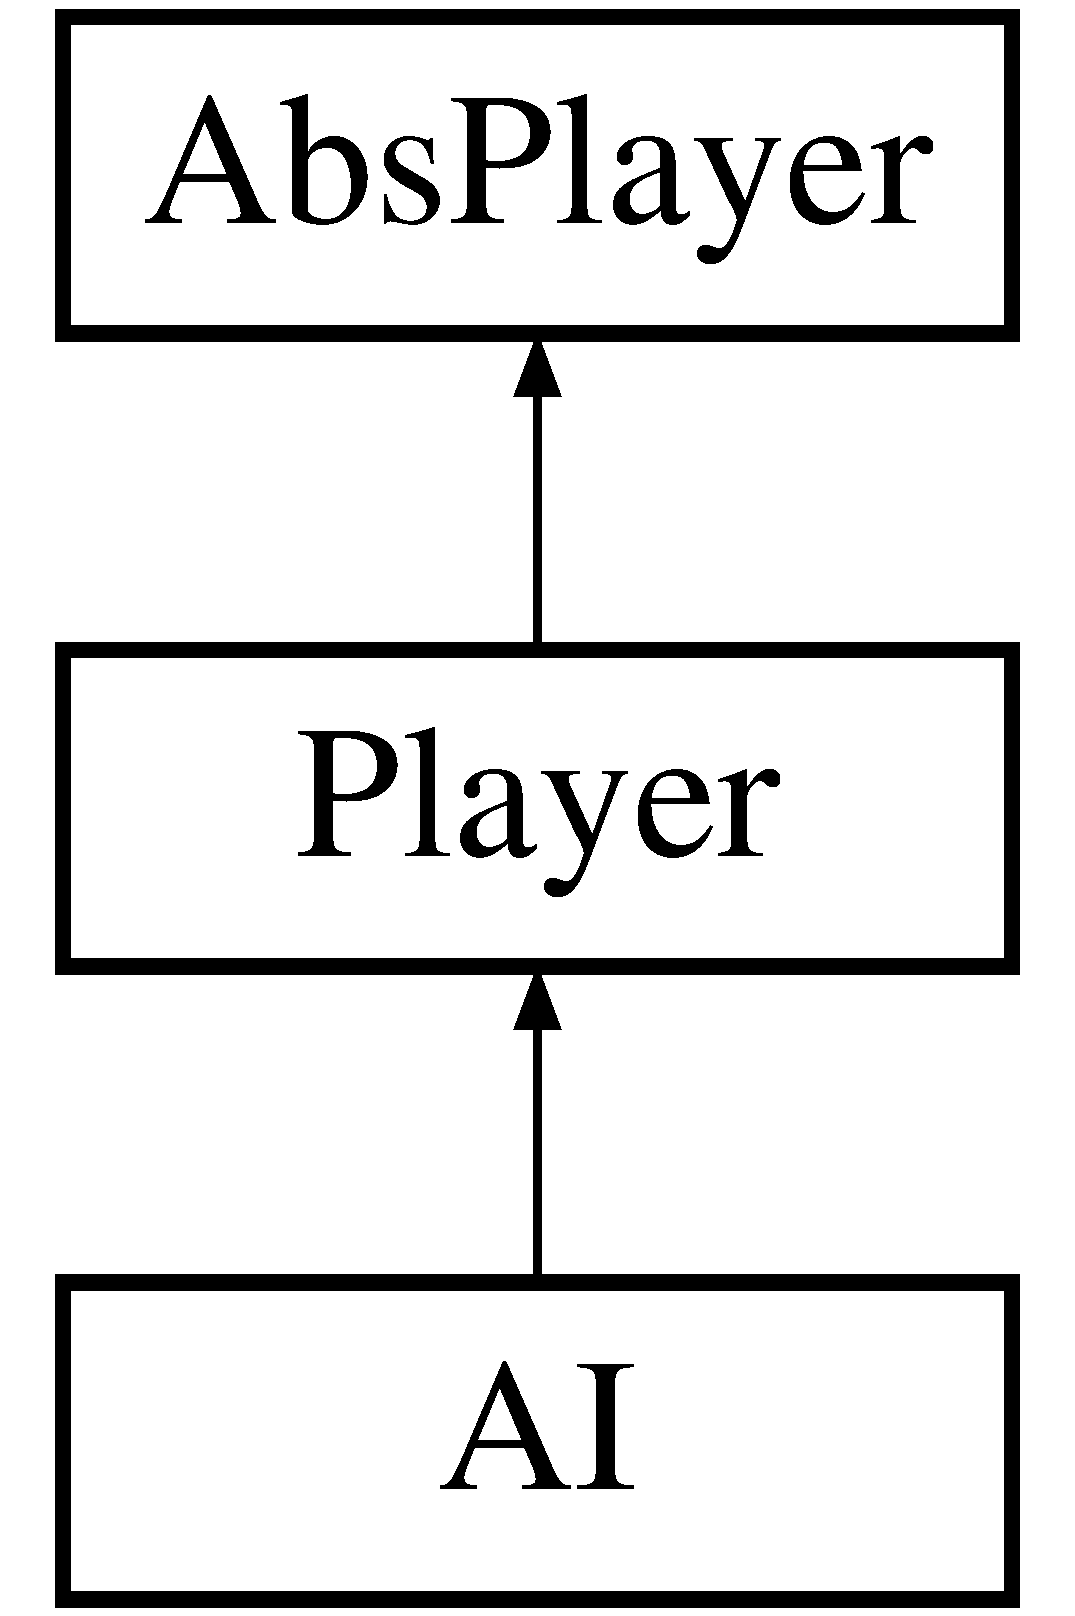
\includegraphics[height=3.000000cm]{class_player}
\end{center}
\end{figure}
\subsection*{Public Member Functions}
\begin{DoxyCompactItemize}
\item 
\hypertarget{class_player_a015ea21fa1e7273e47d48cb20d9b12e3}{}void {\bfseries init} ()\label{class_player_a015ea21fa1e7273e47d48cb20d9b12e3}

\item 
\hypertarget{class_player_adf643edc00fc1718c1fbb34b3693ca78}{}void {\bfseries chalng} ()\label{class_player_adf643edc00fc1718c1fbb34b3693ca78}

\item 
\hypertarget{class_player_afaedda878ae614e71ed711a5b2bc0967}{}void {\bfseries bid} ()\label{class_player_afaedda878ae614e71ed711a5b2bc0967}

\item 
\hypertarget{class_player_af5a03535109b8f5c1a403cb5a4175f42}{}void {\bfseries roll} ()\label{class_player_af5a03535109b8f5c1a403cb5a4175f42}

\item 
\hypertarget{class_player_a78d6a5df3a6dc042a39f8ffe8b6b570e}{}void {\bfseries set\+Ordr} (int n)\label{class_player_a78d6a5df3a6dc042a39f8ffe8b6b570e}

\item 
\hypertarget{class_player_afd1ae6430f71864ab3289d1d00bd9deb}{}void {\bfseries set\+Name} (string s)\label{class_player_afd1ae6430f71864ab3289d1d00bd9deb}

\item 
\hypertarget{class_player_aa6c5e0dd054a620f9a1f8070c3b3cfc3}{}void {\bfseries set\+P\+W} (string)\label{class_player_aa6c5e0dd054a620f9a1f8070c3b3cfc3}

\item 
\hypertarget{class_player_a1d148613cd3164d31114e48525f59da6}{}void {\bfseries set\+Em} (string e)\label{class_player_a1d148613cd3164d31114e48525f59da6}

\item 
\hypertarget{class_player_a91eb5ff686390a15d8805001992cdd02}{}void {\bfseries set\+Info} (\hyperlink{struct_info}{Info} i)\label{class_player_a91eb5ff686390a15d8805001992cdd02}

\item 
\hypertarget{class_player_a9e0cf9b16c393adc49534202e392a49f}{}void {\bfseries set\+Coin} (int c)\label{class_player_a9e0cf9b16c393adc49534202e392a49f}

\item 
\hypertarget{class_player_a433926989957da76385fbc37e732bcf0}{}void {\bfseries set\+Info} (string, string, string)\label{class_player_a433926989957da76385fbc37e732bcf0}

\item 
\hypertarget{class_player_abe9f17c654709de1a7afacc7efedfd7e}{}void {\bfseries add\+Coin} ()\label{class_player_abe9f17c654709de1a7afacc7efedfd7e}

\item 
\hypertarget{class_player_a36d5a5057ee3f62702aaa78809973503}{}void {\bfseries dest\+Vec} ()\label{class_player_a36d5a5057ee3f62702aaa78809973503}

\item 
\hypertarget{class_player_aaa79bb23e3f6f193d101d49ec3f1b36b}{}unsigned int {\bfseries get\+P\+W} () const \label{class_player_aaa79bb23e3f6f193d101d49ec3f1b36b}

\item 
\hypertarget{class_player_a77a2e63cfed717ce18b978b1cb89b1e0}{}int {\bfseries get\+Ordr} () const \label{class_player_a77a2e63cfed717ce18b978b1cb89b1e0}

\item 
\hypertarget{class_player_ab7164df826d0d2048fe653ca699f50d2}{}int {\bfseries get\+Open} () const \label{class_player_ab7164df826d0d2048fe653ca699f50d2}

\item 
\hypertarget{class_player_a5380a48bc89f9624405632be0d4188ab}{}int {\bfseries get\+Num\+P} () const \label{class_player_a5380a48bc89f9624405632be0d4188ab}

\item 
\hypertarget{class_player_a98dc67318971c5063fa9ef58b67040ef}{}int {\bfseries get\+Num} () const \label{class_player_a98dc67318971c5063fa9ef58b67040ef}

\item 
\hypertarget{class_player_ac24ac3e4bf79639ac4823684685acc4b}{}int {\bfseries get\+Coin} () const \label{class_player_ac24ac3e4bf79639ac4823684685acc4b}

\item 
\hypertarget{class_player_ae9edaa4238cee3014ee20758da46f39f}{}int {\bfseries get\+Rond} () const \label{class_player_ae9edaa4238cee3014ee20758da46f39f}

\item 
\hypertarget{class_player_aa2530cc97759ae72f7b21e127d042f66}{}\hyperlink{classa_vector}{a\+Vector}$<$ char $>$ {\bfseries get\+Dice} () const \label{class_player_aa2530cc97759ae72f7b21e127d042f66}

\item 
\hypertarget{class_player_a2df84f2e1b3cfda858df2b5c98957965}{}char {\bfseries get\+Face} () const \label{class_player_a2df84f2e1b3cfda858df2b5c98957965}

\item 
\hypertarget{class_player_a3e55942283c2b94d5434ac80f58d107a}{}\hyperlink{struct_info}{Info} {\bfseries get\+Info} () const \label{class_player_a3e55942283c2b94d5434ac80f58d107a}

\item 
\hypertarget{class_player_a15e4d6563f7a8eca0fc2176d82abbc51}{}bool {\bfseries get\+Wild} () const \label{class_player_a15e4d6563f7a8eca0fc2176d82abbc51}

\item 
\hypertarget{class_player_a213107158b26525b33ee41893c0f3607}{}string {\bfseries get\+Name} () const \label{class_player_a213107158b26525b33ee41893c0f3607}

\item 
\hypertarget{class_player_ab6a7db97f5ff9bc3687cb19011751330}{}string {\bfseries get\+Em} () const \label{class_player_ab6a7db97f5ff9bc3687cb19011751330}

\item 
\hypertarget{class_player_ac30b21b3a1f923138c42daa3e7261f6b}{}int {\bfseries get\+Quan} ()\label{class_player_ac30b21b3a1f923138c42daa3e7261f6b}

\item 
\hypertarget{class_player_af00720c6458ae3cdc554d61f732af880}{}void {\bfseries pnt\+Dice} ()\label{class_player_af00720c6458ae3cdc554d61f732af880}

\item 
\hypertarget{class_player_a9610c874d118eaaf5e36b9f1326bf365}{}void {\bfseries renew\+Fl} (string, int)\label{class_player_a9610c874d118eaaf5e36b9f1326bf365}

\end{DoxyCompactItemize}
\subsection*{Static Public Member Functions}
\begin{DoxyCompactItemize}
\item 
\hypertarget{class_player_a14c0aeb69509335a4e91a0b49d103bf1}{}static void {\bfseries set\+Num\+P} (int n)\label{class_player_a14c0aeb69509335a4e91a0b49d103bf1}

\item 
\hypertarget{class_player_a1476aaca70e47b36c20266d714ab6518}{}static void {\bfseries set\+Num\+C} ()\label{class_player_a1476aaca70e47b36c20266d714ab6518}

\item 
\hypertarget{class_player_a1af5d39f7bac2aeaa1e30c7dda2332fa}{}static void {\bfseries reset} ()\label{class_player_a1af5d39f7bac2aeaa1e30c7dda2332fa}

\item 
\hypertarget{class_player_aab4d4f2f0e6e7249aaa0b03b82844fb1}{}static void {\bfseries set\+Open} (int n)\label{class_player_aab4d4f2f0e6e7249aaa0b03b82844fb1}

\item 
\hypertarget{class_player_a0afc5317b14978b06caf4df9dfdef58c}{}static void {\bfseries set\+Num} (int n)\label{class_player_a0afc5317b14978b06caf4df9dfdef58c}

\item 
\hypertarget{class_player_abbeccad95b0cf837fc589bdb7fae36b9}{}static void {\bfseries set\+Face} (char c)\label{class_player_abbeccad95b0cf837fc589bdb7fae36b9}

\item 
\hypertarget{class_player_a213e2ef93da1ea5e5c5a9891c5b1d14e}{}static void {\bfseries set\+Rond} (int r)\label{class_player_a213e2ef93da1ea5e5c5a9891c5b1d14e}

\item 
\hypertarget{class_player_a992ec6a8d5cbc971b38d87cf0232a5de}{}static void {\bfseries set\+L\+Bdr} (int l)\label{class_player_a992ec6a8d5cbc971b38d87cf0232a5de}

\item 
\hypertarget{class_player_ab5deb6987c7972da5ac4b15cc73ed0fe}{}static int {\bfseries get\+L\+Bdr} ()\label{class_player_ab5deb6987c7972da5ac4b15cc73ed0fe}

\end{DoxyCompactItemize}
\subsection*{Protected Member Functions}
\begin{DoxyCompactItemize}
\item 
\hypertarget{class_player_a391f0c68fe2c4c447cad450696b6a635}{}\hyperlink{classa_vector}{a\+Vector}$<$ char $>$ {\bfseries rol\+Dice} (int)\label{class_player_a391f0c68fe2c4c447cad450696b6a635}

\item 
\hypertarget{class_player_a0040cf1aaccc194845c2b41bec062248}{}void {\bfseries sign} ()\label{class_player_a0040cf1aaccc194845c2b41bec062248}

\item 
\hypertarget{class_player_aed39d90aa1fc67c634a3c39711311067}{}int {\bfseries get\+N\+Inf} ()\label{class_player_aed39d90aa1fc67c634a3c39711311067}

\item 
\hypertarget{class_player_aff6552271f8ee023f5a20dfe72877647}{}void {\bfseries set\+N\+Inf} (int)\label{class_player_aff6552271f8ee023f5a20dfe72877647}

\item 
\hypertarget{class_player_a3dd831a23b52bbea2f77fe40b0de23e6}{}void {\bfseries wt\+File} (\hyperlink{struct_info}{Info} $\ast$, int)\label{class_player_a3dd831a23b52bbea2f77fe40b0de23e6}

\item 
\hypertarget{class_player_acaf05123cef3c79f116077df641b91bb}{}void {\bfseries rd\+File} (\hyperlink{struct_info}{Info} $\ast$, int)\label{class_player_acaf05123cef3c79f116077df641b91bb}

\item 
\hypertarget{class_player_abe7e1ad07be484fcb33342c4d00d6f2c}{}bool {\bfseries valid\+C\+C} (string, int)\label{class_player_abe7e1ad07be484fcb33342c4d00d6f2c}

\end{DoxyCompactItemize}
\subsection*{Static Protected Member Functions}
\begin{DoxyCompactItemize}
\item 
\hypertarget{class_player_ada4b9f7e789e35b7ed9a76d3ddefd33d}{}static void {\bfseries renew} (char, int, bool)\label{class_player_ada4b9f7e789e35b7ed9a76d3ddefd33d}

\end{DoxyCompactItemize}
\subsection*{Protected Attributes}
\begin{DoxyCompactItemize}
\item 
\hypertarget{class_player_a4c5726c0fa6d1e409a03a0ed2a5d765c}{}int {\bfseries order}\label{class_player_a4c5726c0fa6d1e409a03a0ed2a5d765c}

\item 
\hypertarget{class_player_a6e10cf298d1dcb3dea7cc0a18cdf4754}{}\hyperlink{classa_vector}{a\+Vector}$<$ char $>$ {\bfseries dices}\label{class_player_a6e10cf298d1dcb3dea7cc0a18cdf4754}

\end{DoxyCompactItemize}
\subsection*{Static Protected Attributes}
\begin{DoxyCompactItemize}
\item 
\hypertarget{class_player_a1543aaf6b241f8bdf8ca6f8a647bf2d9}{}static int {\bfseries open} =-\/1\label{class_player_a1543aaf6b241f8bdf8ca6f8a647bf2d9}

\item 
\hypertarget{class_player_ad405eb8c39222c17a988993246a00cfb}{}static int {\bfseries num\+Plyr} =0\label{class_player_ad405eb8c39222c17a988993246a00cfb}

\item 
\hypertarget{class_player_a6bd02f63faf1415162da9539e107f12a}{}static int {\bfseries num\+Cd}\label{class_player_a6bd02f63faf1415162da9539e107f12a}

\item 
\hypertarget{class_player_a68a72e6cf75e11bdd6f196a9d81fadc7}{}static char {\bfseries face\+Cd} =\textquotesingle{}0\textquotesingle{}\label{class_player_a68a72e6cf75e11bdd6f196a9d81fadc7}

\item 
\hypertarget{class_player_adc8ed55c08d7ba0393cb806dea68f414}{}static int {\bfseries round} =0\label{class_player_adc8ed55c08d7ba0393cb806dea68f414}

\item 
\hypertarget{class_player_a0aa0b4001546e75caa519dcd68ff8200}{}static bool {\bfseries wild} =true\label{class_player_a0aa0b4001546e75caa519dcd68ff8200}

\item 
\hypertarget{class_player_ad4714edb523a78432863fc7e7521dc59}{}static int {\bfseries last\+Bdr} =-\/1\label{class_player_ad4714edb523a78432863fc7e7521dc59}

\end{DoxyCompactItemize}


\subsection{Detailed Description}


Definition at line 16 of file Player.\+h.



The documentation for this class was generated from the following files\+:\begin{DoxyCompactItemize}
\item 
Player.\+h\item 
Player.\+cpp\end{DoxyCompactItemize}

%--- End generated contents ---

% Index
\backmatter
\newpage
\phantomsection
\clearemptydoublepage
\addcontentsline{toc}{chapter}{Index}
\printindex

\end{document}
